\documentclass[12pt,fleqn]{article}

\usepackage{fullpage}
\usepackage{caption}
\usepackage[round]{natbib}
\usepackage{multirow}
\usepackage{booktabs}
\usepackage{tabularx}
\usepackage{tcolorbox}
\usepackage{graphicx}
\usepackage{float}
\usepackage{hyperref}
\usepackage{color, soul}
\hypersetup{
    colorlinks = true,
    citecolor=black,
    filecolor=black,
    linkcolor=blue,
    urlcolor=red
}
\oddsidemargin 0mm
\evensidemargin 0mm
\textwidth 160mm
\textheight 200mm

\usepackage{fancyhdr}
\fancyhead[L]{March 29, 2018}
\fancyhead[C]{SE 3A04: D3}
\fancyhead[R]{Group 3}
\setlength{\headheight}{52pt}
\renewcommand{\headrulewidth}{0.2pt}

\pagestyle{fancy}
\usepackage[margin=2.5cm,headsep=.2in ]{geometry}

\pagenumbering{arabic}
\newcounter{stepnum}


\title{3A04 Group 3: FIA\\ Detailed Design}

\author{
Dalip Jandir\\
	\texttt{400012917}
	\\
	\\
	\\
	\\
\and
Kathryn Kodama\\
  	\texttt{400013582}
  	\\
  	\\
\and
Tongfei Wang\\
	\texttt{1437618}
\and
Mariah Janet Lindsay\\
    \texttt{1413072}	
    \\
	    \includegraphics[scale=0.2]{img/my_SIGT.png}
	\\
\and
Christopher Cagna\\
    \texttt{001161005}
    \\
    \includegraphics[scale=0.4]{img/,.PNG}
    \\
}

\date{\today\\ Version 1.0}

\begin{document}

\maketitle
\pagebreak
\tableofcontents

\begin{table}[ht]
\caption{\bf Revision History}
\begin{tabularx}{\textwidth}{|p{3cm}|p{2cm}|X|}
\toprule {\bf Version} & {\bf Date} & {\bf Notes}\\
\midrule
1.0 & 20/03/2018 & Created and updated document \\
1.0 & 29/03/2018 & Finalized document for revision 1 \\
\bottomrule
\end{tabularx}
\end{table}
\pagebreak

\section{Introduction}
\subsection{Purpose}
The purpose of this detailed design document is to provide guidance for the architecture of the Flag Identification (FIA) system.  This document details how each aspect of the system communicates with one another and the fine details needed to implement the application.  This document serves as a detailed reference for the developers of the application to utilize throughout implementation. This document can also be referenced throughout testing of the application.

\subsection{System Description}
The system’s primary function is flag identification.  The system will allow the user to upload an image of a flag through their Android Smartphone. The information will be handled by three system experts; colour expert, graph expert and GPS expert. With the help of the three experts, the system will be able to present the user with six flags that best match the flag uploaded. The user will be able to select which of the returned flags, if any, match their uploaded image. The application will allow the user to view their previously searched flags.  Additionally, the application will allow users to see the most searched for flags across all users.

\subsection{Overview}
The following sections detail in-depth implementation details.  Section 2 contains the state charts for each controller class in the FIA system; the View Controller, Forum Controller, State Controller, Colour Controller and GPS Controller.  Section 3 consists of the sequence diagrams corresponding to the FIA system and the use cases detailed in the High-Level Architectural Design document.  Section 4 details the detailed class diagram of the system.  Appendix A details how each member of the development team contributed to the document.

\section{State Charts for Controller Classes}
\subsection{View Controller}
\begin{figure}[H]
    \centering
    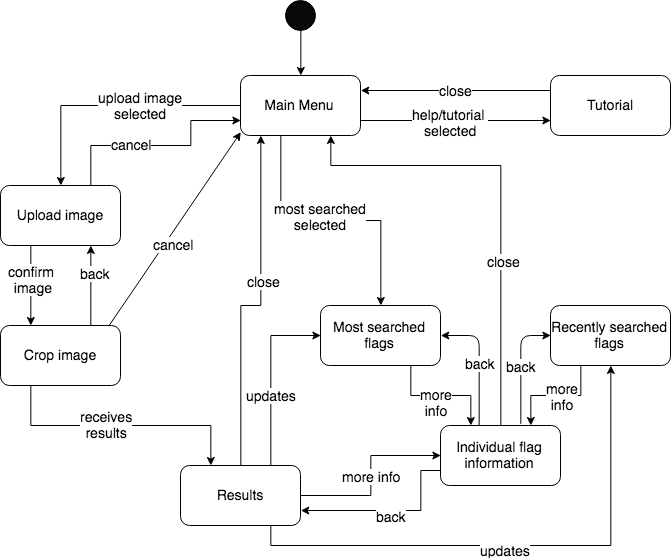
\includegraphics[scale=0.6]{img/View_Controller.png}
    \caption{State chart for View Controller}
\end{figure}

\subsection{Forum Controller}
\begin{figure}[H]
    \centering
    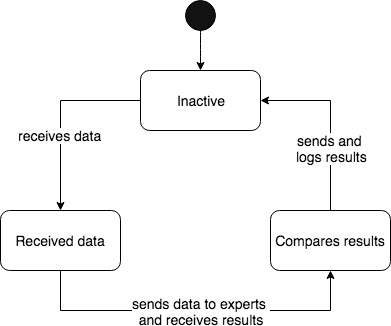
\includegraphics[scale=0.6]{img/Forum_Controller.png}
    \caption{State chart for Forum Controller}
\end{figure}

\subsection{Shape Controller}
\begin{figure}[H]
    \centering
    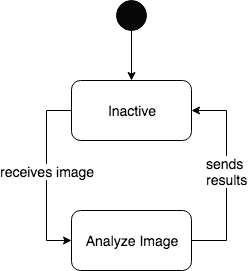
\includegraphics[scale=0.6]{img/Shape_Controller.png}
    \caption{State chart for Shape Controller}
\end{figure}

\subsection{Colour Controller}
\begin{figure}[H]
    \centering
    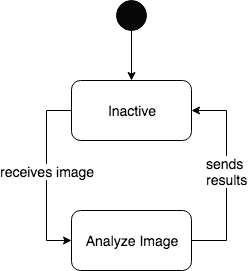
\includegraphics[scale=0.5]{img/Colour_Controller.png}
    \caption{State chart for Colour Controller}
\end{figure}

\subsection{GPS Controller}
\begin{figure}[H]
    \centering
    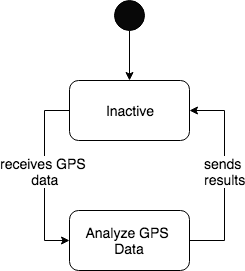
\includegraphics[scale=0.6]{img/GPS_Controller.png}
    \caption{State chart for GPS Controller}
\end{figure}

\newpage
\section{Sequence Diagrams}
Following are the sequence diagrams for each use case in the FIA system.
\subsection{Use Case 1: Navigating to the Most Searched Flags Page}
\begin{figure}[H]
    \centering
    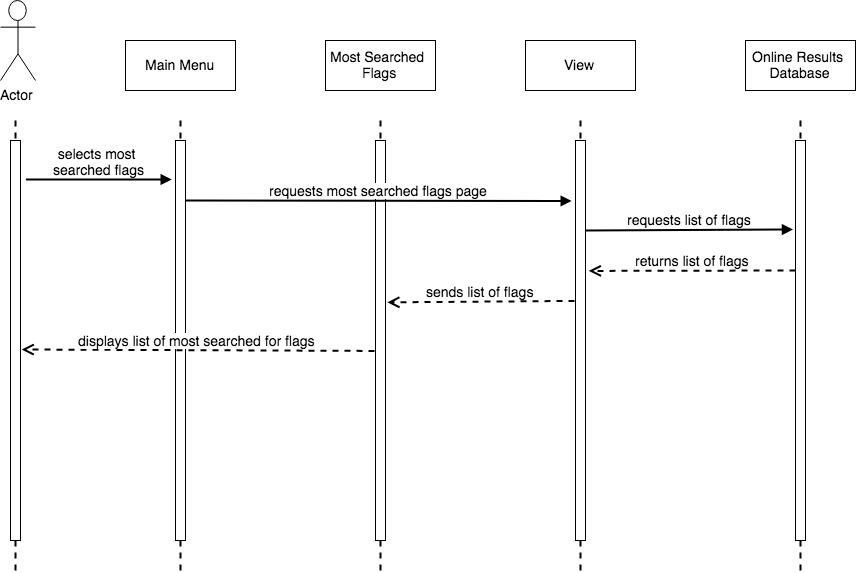
\includegraphics[scale=0.45]{img/SD2.png}
    \caption{Sequence diagram for navigating to the most searched flags page}
\end{figure}

\subsection{Use Case 2: Navigating to the Previous Results Page}
\begin{figure}[H]
    \centering
    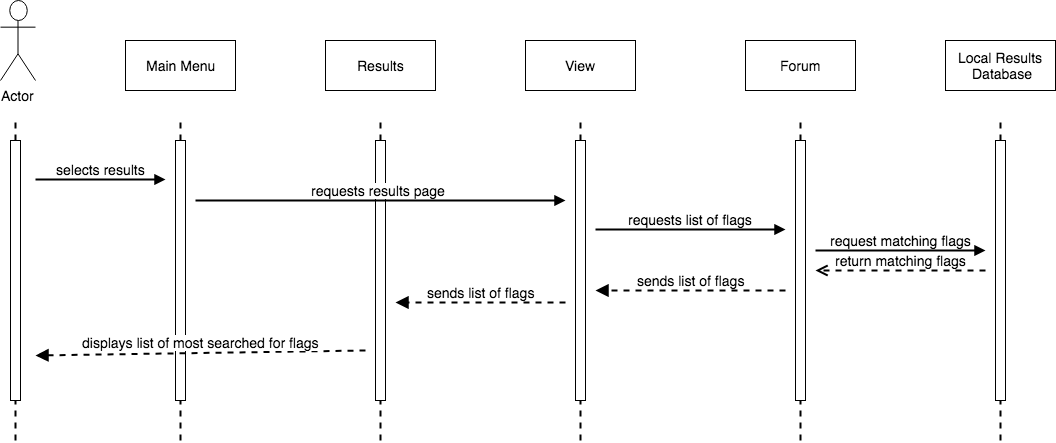
\includegraphics[scale=0.44]{img/SD3.png}
    \caption{Sequence diagram for navigating to the previous results page}

\end{figure}
\subsection{Use Case 3: Identifying a Flag}
\begin{figure}[H]
    \centering
    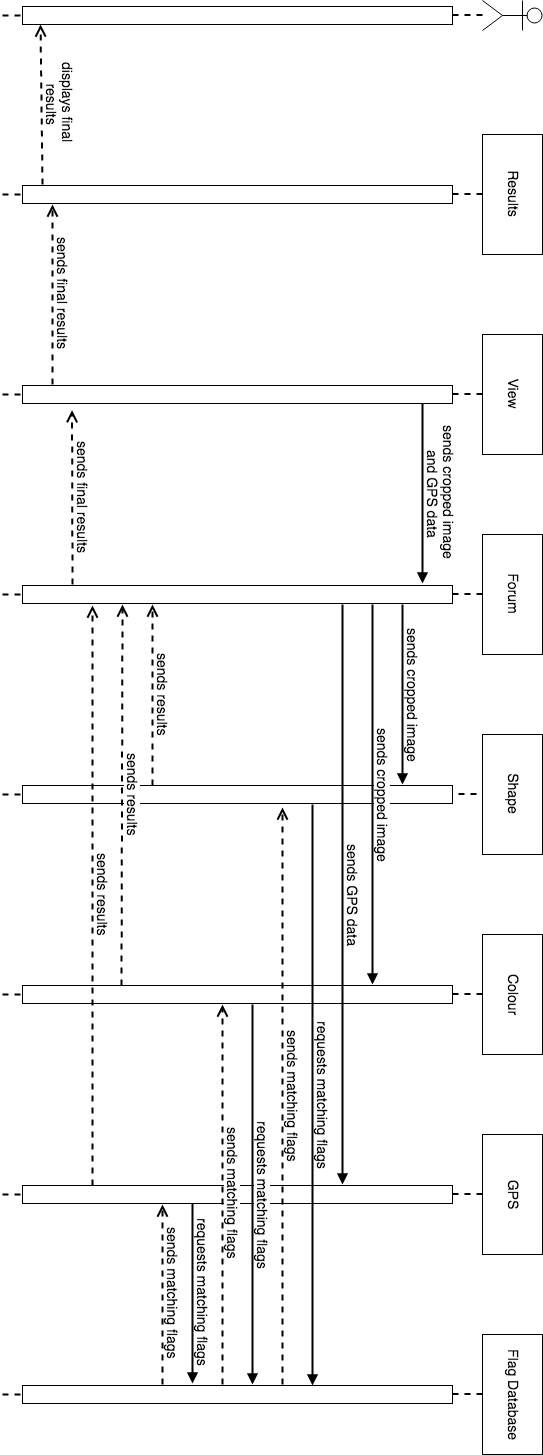
\includegraphics[scale=0.4]{img/SD1.png}
    \caption{Sequence diagram for identifying a flag}
\end{figure}



\subsection{Use Case 4: More Information from the Previous Results Page}
\begin{figure}[H]
    \centering
    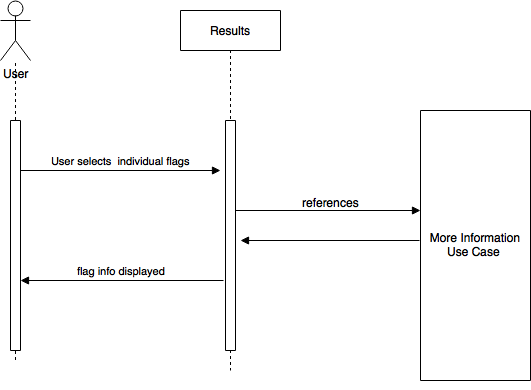
\includegraphics[scale=0.6]{img/SD4.png}
    \caption{Sequence diagram for the user requesting more information on an individual flag from the previous results page}
\end{figure}

\subsection{Use Case 5: More Information from the Most Searched Flags Page}
\begin{figure}[H]
    \centering
    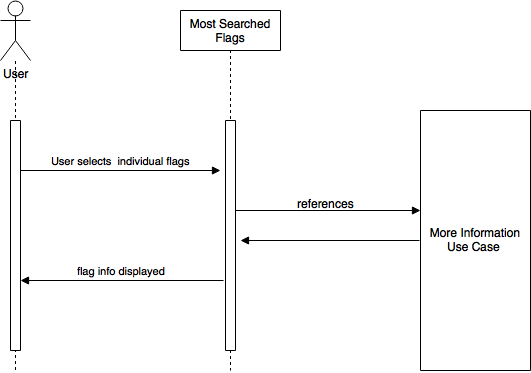
\includegraphics[scale=0.6]{img/SD5.png}
    \caption{Sequence diagram for the user requesting more information on an individual flag from the most searched flags page}
\end{figure}


\subsection{Use Case 6: More Information on a Flag}
\begin{figure}[H]
    \centering
    \includegraphics[scale=0.3]{img/SD6.png}
    \caption{Sequence diagram for viewing more information on an individual flag}
\end{figure}

\subsection{Use Case 7: User Uploads an Image}
\begin{figure}[H]
    \centering
    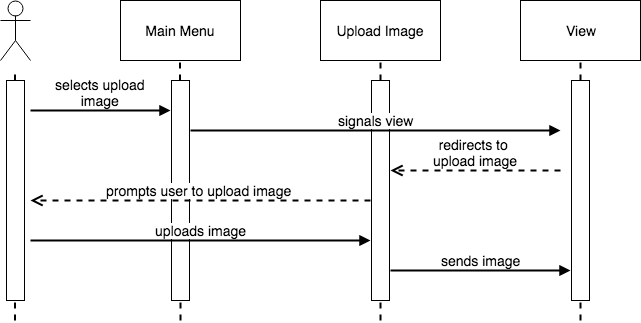
\includegraphics[scale=0.6]{img/SD7.png}
    \caption{Sequence diagram for the user uploading an image}
\end{figure}

\subsection{Use Case 8: User Crops an Image}
\begin{figure}[H]
    \centering
    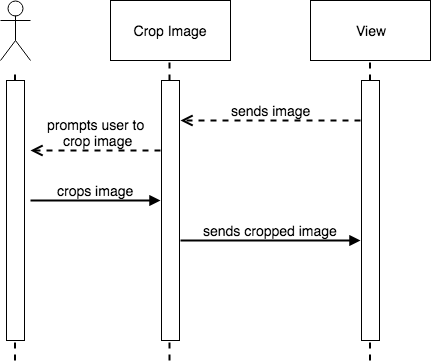
\includegraphics[scale=0.6]{img/SD8.png}
    \caption{Sequence diagram for the user cropping an image}
\end{figure}

\subsection{Use Case 9: User Selects the Correct Result}
\begin{figure}[H]
    \centering
    \includegraphics[scale=0.5]{img/SD9.png}
    \caption{Sequence diagram for the user selecting the correct result}
\end{figure}


\section{Detailed Class Diagram}
\begin{figure}[H]
    \centering
    \includegraphics[scale=0.5]{img/ClassDiagram.png}
    \caption{UML Class Diagram for the FIA System}
\end{figure}
\newpage
\appendix
\section{Division of Labour}
\begin{itemize}
    \item Section 1.1: Kathryn Kodama
    \item Section 1.2: Christopher Cagna, Dalip Jandir
    \item Section 1.3: Mariah Janet Lindsay, Tongfei Wang
    \item Section 2: Christopher Cagna, Dalip Jandir, Kathryn Kodama, Mariah Janet Lindsay, Tongfei Wang
    \item Section 3:  Christopher Cagna, Dalip Jandir, Kathryn Kodama, Mariah Janet Lindsay, Tongfei Wang
    \item Section 4:  Christopher Cagna, Dalip Jandir, Kathryn Kodama, Tongfei Wang
    
\end{itemize}
\end{document}